\documentclass[11pt,a4paper]{article}
\usepackage{termpaper}
\usepackage[utf8]{inputenc} 
\usepackage[ngerman]{babel}
\usepackage{graphicx}
\usepackage{listings}
\usepackage{xcolor}
\usepackage{cleveref}
\usepackage{filecontents}
\usepackage{url}
\usepackage[labelfont=bf,textfont=it]{caption}
\usepackage{courier}

\definecolor{lstcolor}{rgb}{0.95,0.95,0.95}

\lstdefinestyle{customc}{
	basicstyle=\footnotesize\ttfamily,
	keywordstyle=\color{black}\bfseries\underbar,
	identifierstyle=,
	commentstyle=\color{white},
	stringstyle=\ttfamily,
	showstringspaces=false,
  	tabsize=2,
	mathescape=true,
	numbers=left,
	numberstyle=\tiny,
	numbersep=10pt,
	captionpos=b,
	frame=trBL,
	breaklines=true
}
\lstset{style=customc}
\renewcommand{\lstlistingname}{Algorithmus}

%opening
\title{Parallele Breitensuche}
\author{
 \authorname{Alexander Gallauner} \\
 \studentnumber{1026090} \\
 \curriculum{534} \\
 \email{alexander.gallauner@gmail.com}
}

\begin{document}
\maketitle
\begin{abstract}
In dieser Arbeit beschäftigen wir uns mit dem Parallelisieren eines bekannten Algorithmus, der Breitensuche (BFS - \textit{Breadth-First Search}). Dabei handelt es sich um einen Suchalgorithmus für Graphen, der in vielen Fragestellungen der Graphentheorie involviert ist. Wir werden uns auf die Parallelisierung dieses Verfahrens auf Rechner mit physikalisch verteiltem Speicher (DMM - \textit{distributed memory machine}) beschränken und mehrere Wege aufweisen, wie man diese Parallelisierung realisieren kann. Dies ist keine leichte Aufgabe, da parallele Abläufe in der sequentiellen Breitensuche nicht sofort ersichtlich sind und ein guter Kompromiss zwischen Speicherverbrauch und Kommunikationsaufwand zwischen Prozessoren gefunden werden muss. Es werden verschiedene Implementierungen der Parallelisierung vorgestellt und anhand verschiedener Kriterien wie Laufzeit, Speedup und Effizienz analysiert. Außerdem wird erklärt, welche Voraussetzungen gelten müssen, damit eine bestimmte Implementierung überhaupt Sinn macht. Die Implementierung findet in der Programmiersprache C statt und zur Kommunikation der Prozessoren untereinander wird OpenMPI verwendet, das eine Open-Source Implementierung des Message Passing Interface Standards (MPI) bereitstellt. (Beispiel für einen erreichten Speedup)\\
Zusätzlich wird das Projekt Graph500 vorgestellt. Graph500 ist ein Benchmark für Supercomputer, die datenintensive Anwendungen ausführen. Da die Breitensuche bei groß angelegten Graphen ein ebenfalls daten- und rechenintensives Problem darstellt, steht diese Suche im Mittelpunkt des Graph500 Projektes. So wie die Implementierungen der parallelen Breitensuche wird auch unsere Implementierung des Graph500 Projektes auf dem Supercomputer Jupiter, ein Rechner der TU Wien mit physikalisch verteiltem Speicher, ausgeführt und analysiert. Innerhalb dieses Projektes wird die Leistung in der Maßeinheit TEPS (\textit{traversed edges per second}) gemessen, welche Auskunft gibt, wie viele Kanten pro Sekunde innerhalb des Graphen besucht werden und wo sich Jupiter anhand des Benchmarks in der Graph500 Rangliste der Supercomputer einordnen würde.
\end{abstract}
\clearpage
\section{Einleitung}
Graphabstraktionen spielen in vielen wissenschaftlichen aber auch alltäglichen Gebieten eine wesentliche Rolle. Viele algorithmische Probleme können auf Graphen zurückgeführt werden, aber auch umgekehrt basiert die Lösung graphentheoretischer Probleme auf Algorithmen. Das Problem der Suche nach dem kürzesten Weg zwischen zwei Orten in einem Straßennetz kann durch einen Graph abstrahiert und mit Hilfe dieses Graphs gelöst werden. Ein Algorithmus, der den kürzesten Weg in einem ungewichteten Graph findet und Thema dieser Bachelorarbeit ist, ist die Breitensuche.\\
Vor über einem halben Jahrhundert wurde der erste Algorithmus, der den Graphen im Prinzip der Breitensuche traversiert, von Moore (REF), während er sich mit der Findung von Pfaden in Labyrinthen beschäftigte, untersucht und herausgebracht. Fast zur gleichen Zeit und unabhängig von der Arbeit von Moore untersuchte Lee (REF) den selben Algorithmus, aber in Bezug auf das Verlegen von Drähten auf einer Platine und die damit verbundene automatische Herstellung von Platinen. Bevor wir mehr auf die Breitensuche eingehen, werden wir zuerst die Eigenschaften eines Graphen genauer beschreiben und die einzelnen Bestandteile erklären und veranschaulichen.\\
Ein Graph in der Graphentheorie ist eine abstrakte Struktur, die eine Menge von Objekten und die Verbindungen zwischen diesen Objekten repräsentiert. Genauer ausgedrückt besteht ein Graph \(G = (V, E)\), wie von Drmota, Gittenberger, Karigl und Panholzer beschrieben,  aus einer endlichen Knotenmenge \(V = V(G)\) und einer endlichen Kantenmenge \(E = E(G)\). Dabei kann eine Kante gerichtet oder ungerichtet sein. Falls alle Kanten gerichtet sind, spricht man auch von einen gerichteten Graphen, andererseits von einem ungerichteten Graphen. In dieser Arbeit arbeiten wir ausschließlich mit ungerichteten Graphen, das heißt jede Kante \(e \in E(G)\) entspricht einem ungeordnetem Paar \(e = \{ v_{1},v_{2} \} = v_{1}v_{2}\) von zwei Knoten \(v_{1}, v_{2} \in V(G)\).
\begin{figure}[h]
 	\centering
	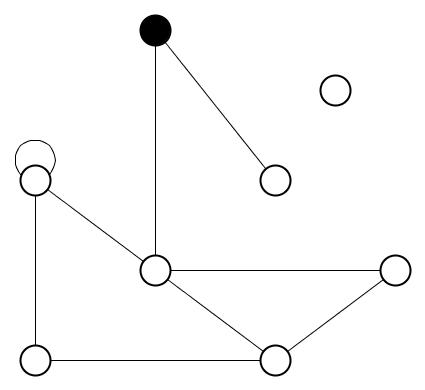
\includegraphics[width=0.5\textwidth]{graph}
 	\caption{Beispiel eines ungerichteten Graphen mit einem Startknoten und einer Schlinge.}
	\label{fig:graph}
\end{figure}
Abbildung~\ref{fig:graph} zeigt ein Beispiel für einen ungerichteten Graphen. Eingezeichnet ist bereits ein Startknoten, schwarzer Knoten, da jede Breitensuche neben dem Graphen einen Start- beziehungsweise Wurzelknoten als Eingabeparameter erwartet. Zusätzlich ist im Graphen eine Schlinge ersichtlich, es sind also auch Kanten zugelassen, bei denen Anfangsknoten gleich Endknoten sind, was innerhalb einer Implementierung der Breitensuche berücksichtigt werden muss. Außerdem kann es sein, dass der Graph nicht zusammenhängend ist und es daher keine Kante zu mindestens einem Knoten gibt. Liegt so ein Graph vor, kann es sein, dass bestimmte Knoten ausgehend vom Startknoten durch die Breitensuche nicht erreicht werden können.\\
Um die Breitensuche zu konkretisieren beziehungsweise besser beschreiben zu können, wird noch der Begriff des Weges und der Distanz zwischen zwei Knoten spezifiziert. Eine Kantenfolge \(e_{1}, e_{2}, ..., e_{k} \in E(G)\) in einem ungerichteten Graphen \(G\) heißt \textit{Weg}, wenn alle Knoten, die durch diese Kantenfolge durchlaufen werden, voneinander verschieden sind. Während die Länge des Weges mit der Anzahl der Kanten zwischen zwei Knoten gleichzusetzen ist, bezeichnet man die \textit{Distanz} zweier Knoten  als den kürzesten Weg zwischen diesen. Das Prinzip der Breitensuche impliziert nun, dass zuerst die Knoten mit der Distanz \(d\) besucht werden und erst in Folge die Knoten mit der Distanz \(d+1\). Dadurch wird der Graph durch die Breitensuche in Levels unterteilt, wobei ein \textit{Level} eine Menge von Knoten definiert, die die selbe Distanz zum Startknoten aufweisen, was in Abbildung~\ref{fig:graph_level} ersichtlich ist. Dabei kann man auch sagen, dass der Knoten die Distanz \(d\) aufweist beziehungsweise zum Level \(d\) gehört. Die größte Distanz zwischen zwei Knoten in einem Graphen \(G\) wird auch als Durchmesser \(D(G)\) (\textit{diameter}) bezeichnet.\\
\begin{figure}[h]
 	\centering
	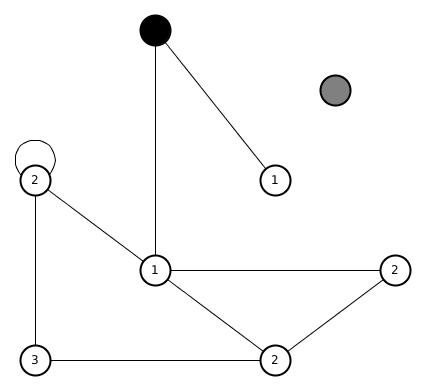
\includegraphics[width=0.5\textwidth]{graph_level}
 	\caption{Nach der Breitensuche ist der Graph in Levels unterteilt. Dies ist ersichtlich an den Distanzen, die in den Knoten eingezeichnet sind. Der graue Knoten entspricht einem nicht besuchten Knoten.}
	\label{fig:graph_level}
\end{figure}
Ausgehend vom Startknoten wurde die Breitensuche auf den Graph von Abbildung~\ref{fig:graph} angewendet. Dadurch wird der Graph in die einzelnen Levels unterteilt, welche aus der Beschriftung der Knoten ersichtlich sind. Der grau hinterlegte Knoten entspricht einem Knoten, der durch die Breitensuche nicht erreicht wurde. Der Durchmesser ist gleich dem höchstem Level im Graphen und ist in diesem Fall \(3\).
Es ist auch möglich andere Informationen als die Distanz in Bezug auf einen Knoten abzuspeichern. Dies wird von vielen unterschiedlichen Applikationen, die die Breitensuche anwenden, erwartet beziehungsweise gefordert. Ein Beispiel dafür ist das Abspeichern des Vaterknotens für jeden besuchten Knoten, damit man am Ende der Breitensuche einen Spannbaum der besuchten Knoten liefern kann. Aus Performancezwecken und auch als Beitrag zur Einfachheit und Parallelität sollten zusätzlichen Informationen oder Berechnungen, wenn möglich, beim erstmaligen Besuchen des Knoten durchgeführt werden.\\
Nachdem die grundlegenden Bestandteile und Eigenschaften eines Graphen geklärt sind, widmen wir uns weiters dem eigentlichen Thema dieser Arbeit, nämlich der Breitensuche. Auch wenn das Grundkonzept der Breitensuche schon erklärt wurde, zeigt Algorithmus~\ref{fifo} eine klassische sequentielle Variante von Cormen, Leiserson, Rivest and Stein \cite{cormen_introduction_2009}, welche eine Warteschlange (\textit{queue}) verwendet, die im FIFO (\textit{first in first out}) Prinzip arbeitet. Diese Variante der Implementierung gehört zu einer der einfachsten der Breitensuche.
\begin{lstlisting}[caption={Klassische Variante der Breitensuche unter Verwendung einer FIFO Warteschlange als Datenstruktur. Wird auf einem Graph \(G\) mit Startknoten \(v_{0} \in V(G)\) angewandt. Der Algorithmus bestimmt die Distanz und den Vaterknoten von denjenigen Knoten, die ausgehend vom Startknoten erreichbar sind.},label=fifo]
$\textbf{SERIAL-BFS}$(G,$v_{0}$)
	$\textbf{for}$ each vertex $\in$ V(G) - {$v_{0}$}
		u.d = $\infty$
		u.$\pi$ = NIL
	$v_{0}$.d = 0
	$v_{0}$.$\pi$ = NIL
	Q = {$v_{0}$}
	$\textbf{while}$ Q $\neq$ 0
		u = DEQUEUE(Q)
		$\textbf{for}$ each v $\in$ G.Adj[u]
			$\textbf{if}$ v.d == $\infty$
				v.d = u.d + 1
				v.$\pi$ = u
				ENQUEUE(Q,v)
\end{lstlisting}
Zu Beginn von Algorithmus~\ref{fifo} werden alle Knoten, die in \(V(G)\) enthalten sind, in den Zeilen 2-4 initialisiert. Ein Knoten \(u \in V\) besitzt die Attribute \lstinline{u.d} für die Distanz und \lstinline{u.$\pi$} für den Vaterknoten. Da zu Beginn noch keine Knoten besucht wurden, wird die Distanz \lstinline{u.d} auf \lstinline{$\infty$} und der Vaterknoten \lstinline{u.$\pi$} auf \lstinline{NIL} gesetzt. Das hat auch folgenden Grund, dass Knoten, die nicht durch die Breitensuche erreicht werden, keine Vaterknoten besitzen, \lstinline{u.$\pi$ = NIL}, und keine gültige Distanz, \lstinline{u.d = $\infty$}, ausgehend vom Startknoten aufweisen.\\
Zeile 5 weist dem Attribut Distanz des Startknotens den Wert 0 zu. In Zeile 6 wird der Vaterknoten des Startknotens auf \lstinline{NIL} gesetzt. In Zeile 7 und 8 wird die Warteschlange initialisiert und bekommt als erstes Element den Startknoten. Nun wird die \lstinline{$\textbf{while}$} Schleife von Zeile 8-14 solange ausgeführt, solange es Knoten gibt, die noch nicht besucht wurden, aber vom Startknoten erreichbar sind. Innerhalb der \lstinline{$\textbf{while}$} Schleife wird in Zeile 9 das Element nach dem FIFO Prinzip aus der Warteschlange genommen, das heißt das Element, das zeitlich am längsten in der Warteschlange war. Die \lstinline{$\textbf{for}$} Schleife in den Zeilen 10-14 iteriert über die Nachbarn \lstinline{v $\in$ G.Adj[u]} des aktuellen Knoten \lstinline{u}. Als Nachbar werden folgende Knoten bezeichnet, die adjazent zum jeweiligen Knoten sind, also durch eine Kante verbunden sind. In Zeile 11 wird überprüft, ob der Knoten \lstinline{v} noch nicht besucht wurde, was mittels \lstinline{$\textbf{if}$} Bedingung
\lstinline{v.d == $\infty$} geprüft wird. Ist dies der Fall, wird \lstinline{v.d} auf \lstinline{u.d + 1} gesetzt und \lstinline{u} wird als Vater in \lstinline{v.$\pi$} gekennzeichnet. Danach wird der Knoten \lstinline{u} in die Warteschlange aufgenommen.
\textbf{Breadth-first trees}
\clearpage

\nocite{*}
\bibliographystyle{abbrv}
\bibliography{bachelor}
\clearpage
\appendix
\section{BFS versions}
\label{sec:versions}
\lstinputlisting[firstline=138,lastline=196,caption={Version 1 - level bitmap},label=version1]{../Source/bfs_par.c}
\lstinputlisting[firstline=135,lastline=183,caption={Version 2 - level array},label=version2]{../Source/bfs_par_parentarray.c}
\lstinputlisting[firstline=153,lastline=205,caption={Version 3 - visited bitmap},label=version3]{../Source/bfs_par_allvisited_parallelsort.c}
\section{Source Code - graph500}
\label{sec:sourcecode}
\lstinputlisting[caption={BFS solution},label=bfs]{../Source/bfs_par_allvisited_parallelsort.c}
\clearpage
\lstinputlisting[caption={Kronecker Generator},label=kronecker_generator]{../Source/kronecker_generator.c}
\clearpage
\lstinputlisting[caption={project.h},label=project]{../Source/project.h}

\clearpage


\end{document}